\section{More Experimental Results}\label{sec:more-experimental-results}
We conducted our experiments on the ImageNet dataset in the same way as in Section~\ref{sec:experiments}.
The only difference is that we used a 50-layer residual network instead of the 110-layer one.
The figures of the Imagenet dataset are consistent with our previous findings on the CIFAR-10 dataset.
\begin{figure}[htbp]
    \centering
    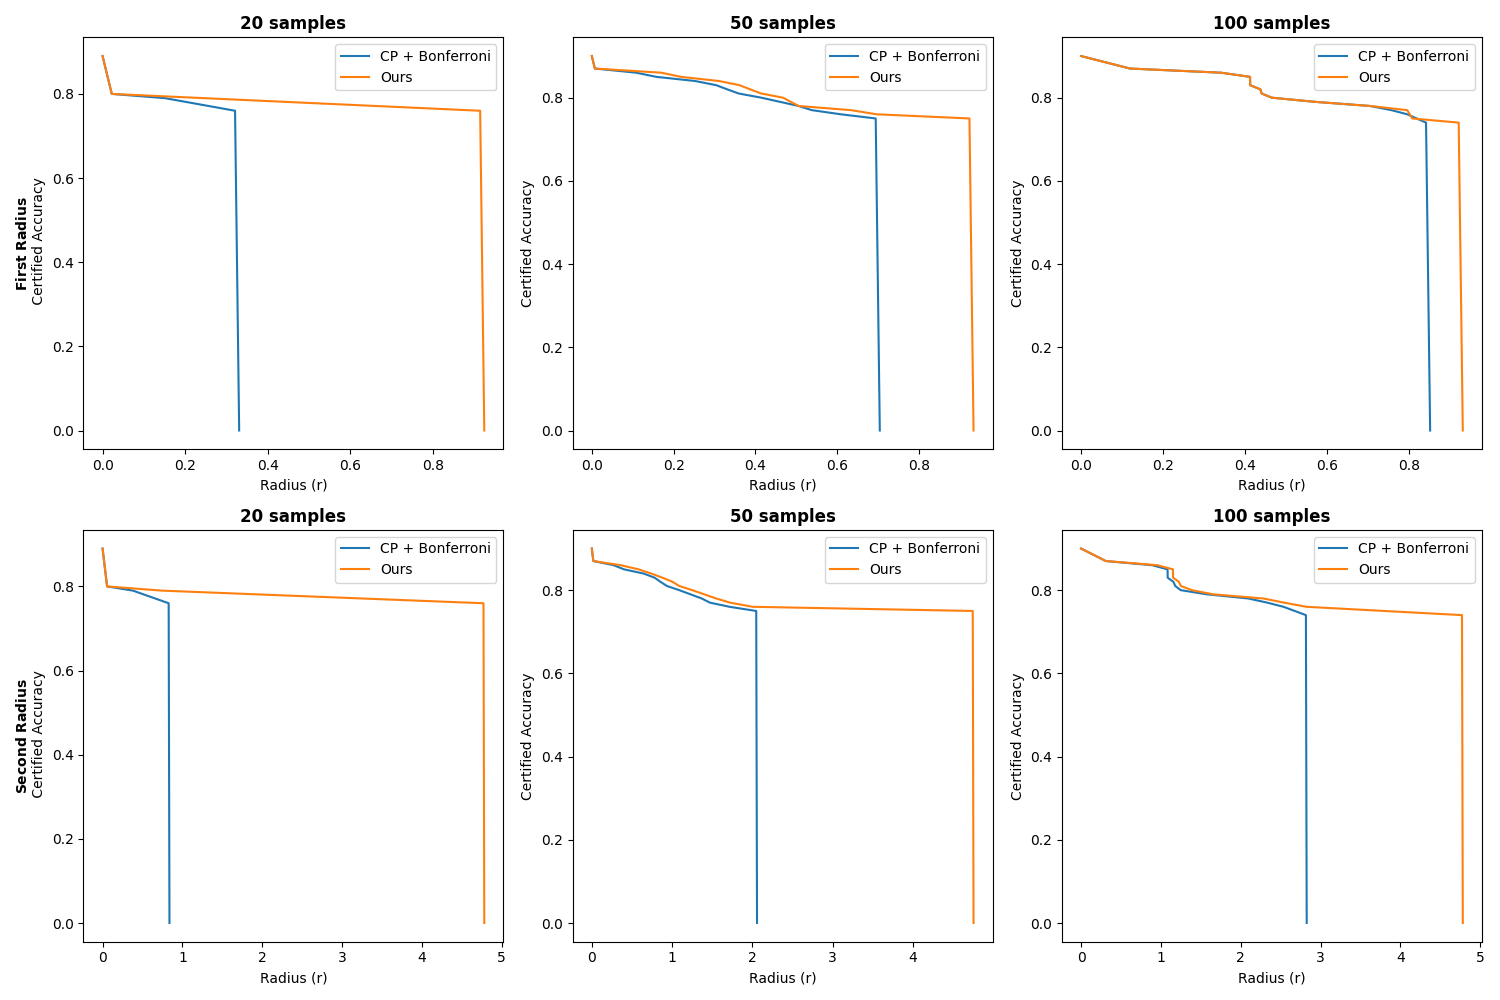
\includegraphics[width=0.8\textwidth]{images/discrete_num_imagenet}
    \caption{Certified accuracies' comparison on the ImageNet dataset in the discrete case for different numbers of samples (displayed on the columns) with $\sigma = 0.25$.}
    \label{fig:discrete_num_imagenet}
\end{figure}
\begin{figure}[htbp]
    \centering
    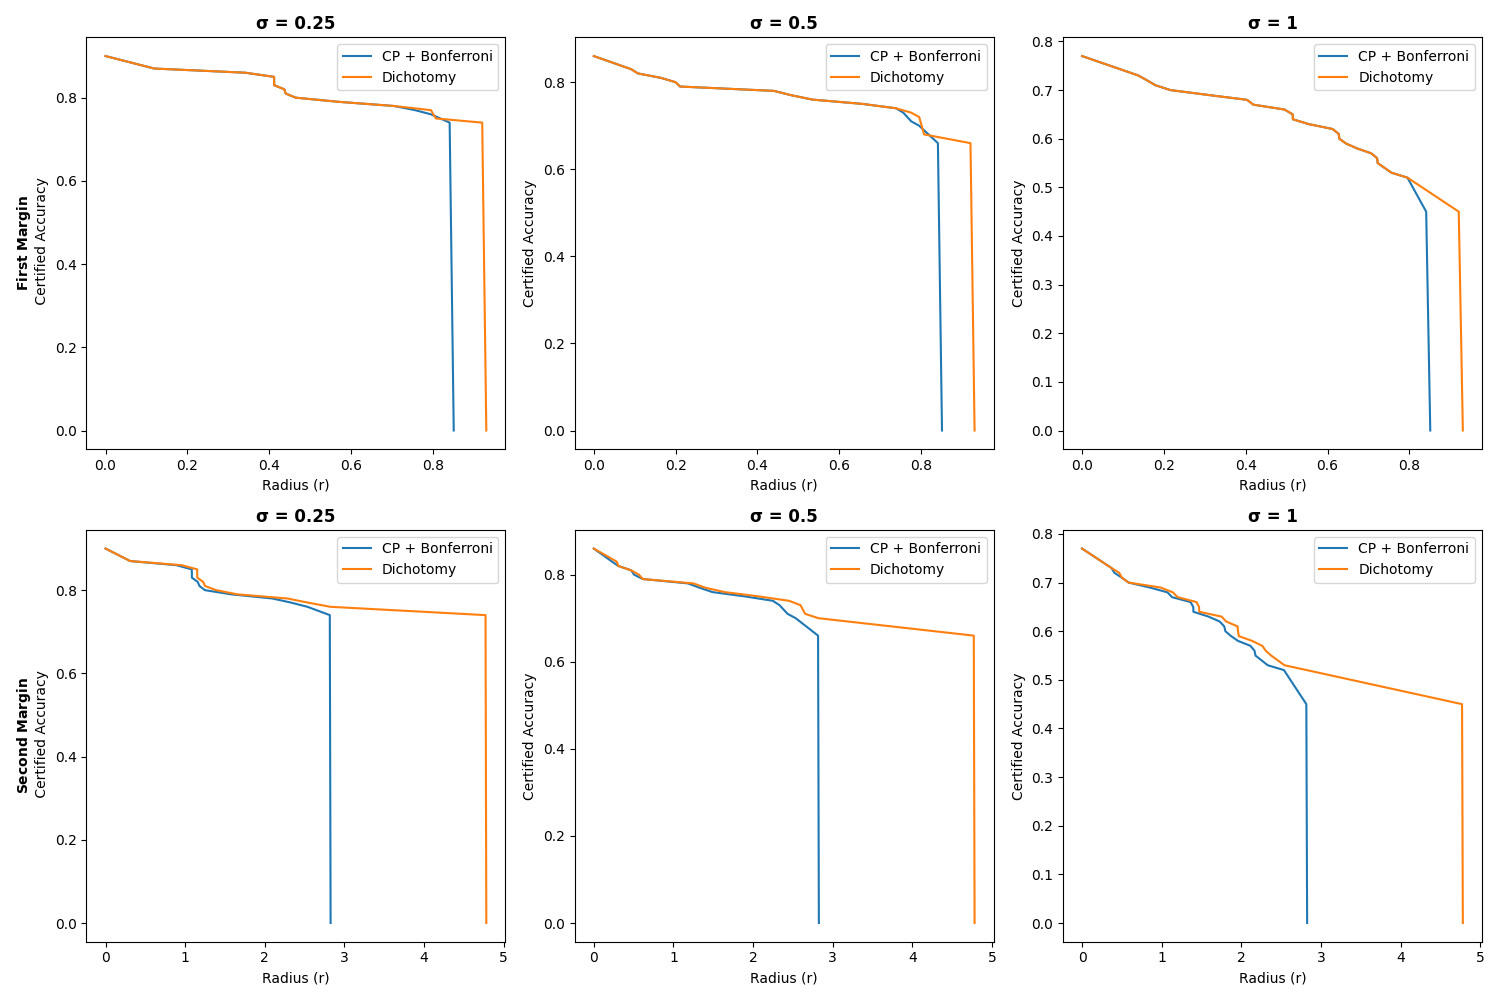
\includegraphics[width=0.8\textwidth]{images/discrete_sigma_imagenet}`
    \caption{Certified accuracies' comparison on the ImageNet dataset in the discrete case for different standard deviations (displayed on the columns) with a sample size of $100$.}
    \label{fig:discrete_sigma_imagenet}
\end{figure}
\begin{figure}[htbp]
    \centering
    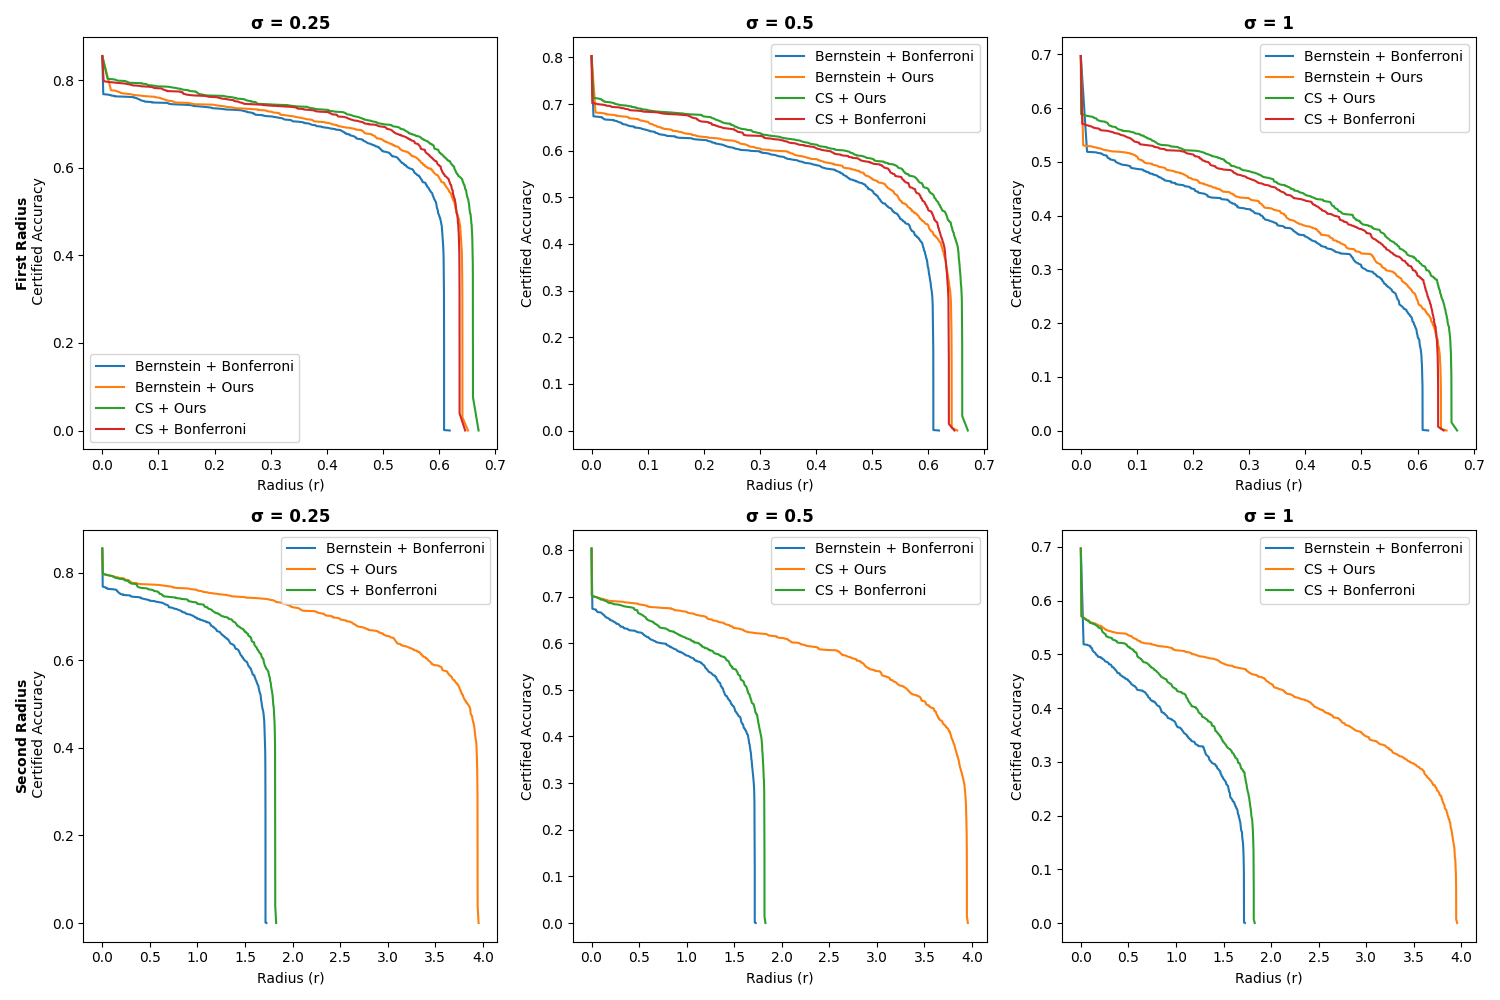
\includegraphics[width=0.8\textwidth]{images/cont_sigma_imagenet}`
    \caption{Certified accuracies' comparison on the ImageNet dataset in the continuous case for different standard deviations (displayed on the columns) with a sample size of $100$ and a temperature equal to $0.5$.}
    \label{fig:cont_sigma_imagenet}
\end{figure}
\begin{figure}[htbp]
    \centering
    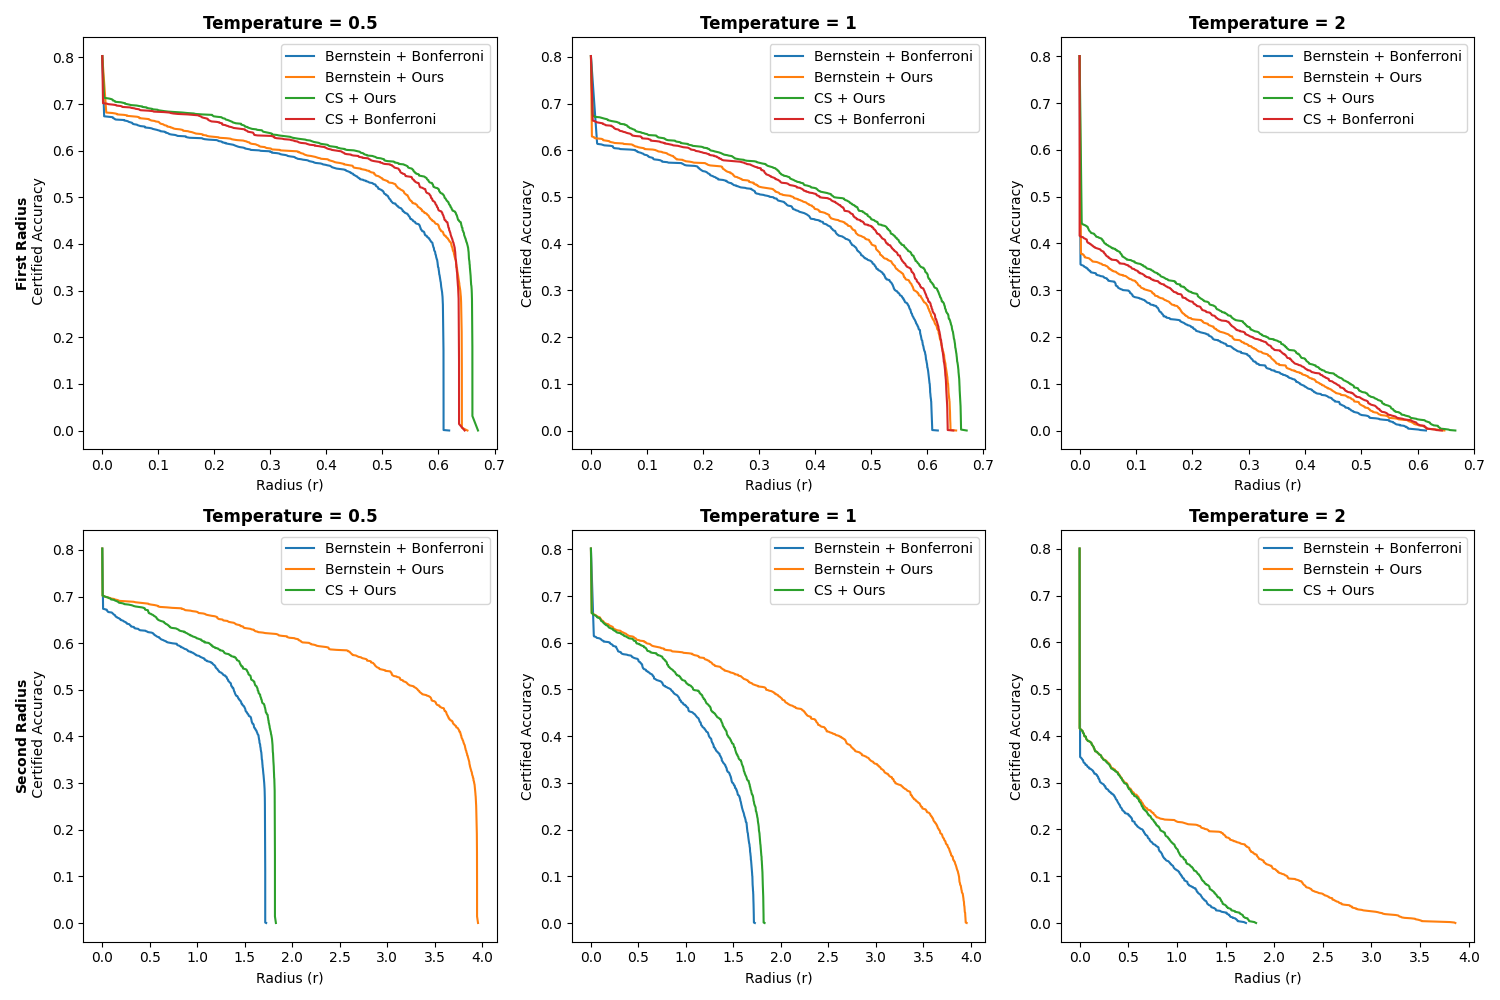
\includegraphics[width=0.8\textwidth]{images/cont_temp_imagenet}
    \caption{Certified accuracies' comparison on the CIFAR-10 dataset in the continuous case for different temperatures (displayed on the columns) with a sample size of $100$ and $\sigma = 0.5$.}
    \label{fig:cont_temp_imagenet}
\end{figure}
